\documentclass[11pt,a4paper]{article}

% ---------- Packages ----------
\usepackage[margin=1in]{geometry}
\usepackage{amsmath,amssymb}
\usepackage{graphicx}
\usepackage{booktabs}
\usepackage{array}
\usepackage{caption}
\usepackage{float}
\usepackage[hidelinks]{hyperref}
\usepackage{enumitem}
\usepackage{fancyhdr}
\usepackage{titlesec}
\usepackage{xcolor}

\titleformat{\section}{\large\bfseries}{\thesection}{1em}{}
\titleformat{\subsection}{\normalsize\bfseries}{\thesubsection}{1em}{}

\pagestyle{fancy}
\fancyhf{}
\fancyhead[L]{Machine-Learning-Based Prediction of Irrigation Water Demand}
\fancyhead[R]{\thepage}
\renewcommand{\headrulewidth}{0.4pt}

\title{\textbf{Machine-Learning-Based Prediction of\\Irrigation Water Demand}\\[0.3em]
\large A Civil Engineering (Water Resources Engineering) Term Project}
\author{Akhil Nistala}
\date{\today}

\begin{document}

\maketitle
\thispagestyle{empty}

\begin{abstract}
\noindent
Efficient irrigation scheduling requires a reliable daily estimate of crop water
demand. This project develops a machine-learning pipeline that predicts daily
gross irrigation water requirement from weather, crop, and antecedent-demand
variables. Because no instrumented field dataset was available, a synthetic but
\emph{physically grounded} dataset (2{,}000 daily records, $\approx$5.5 years) was
generated using the \textbf{FAO-56 Penman--Monteith} reference evapotranspiration
equation, FAO-56 crop coefficients for maize, and the USDA-SCS effective-rainfall
formula, with realistic day-to-day weather variability calibrated to a
representative central-Indian, subtropical-monsoon climate. Three regression
models --- Linear Regression, Decision Tree, and Random Forest --- were trained
on an 80/20 \textbf{chronological} split and evaluated using MAE, RMSE, and
R\textsuperscript{2}. Random Forest achieved the best performance
(R\textsuperscript{2} $\approx$ 0.97, MAE $\approx$ 0.42~mm/day), substantially
outperforming Linear Regression (R\textsuperscript{2} $\approx$
0.92, MAE $\approx$ 0.72~mm/day), consistent with the expectation that irrigation
demand depends on nonlinear interactions between weather variables, crop
coefficient, and rainfall. A \textbf{three-metric feature-importance analysis}
(correlation with target, Random Forest impurity-based importance, and
permutation importance on the held-out test set) was carried out to
cross-validate which inputs actually drove the predictions, rather than relying
on a single importance measure. Results were checked for physical reasonableness
against known Indian agro-climatic irrigation patterns and found consistent.
\end{abstract}

\vspace{1em}

\section{Problem Statement}

Irrigation water is a scarce and expensive resource, and over- or
under-irrigation both carry costs: over-irrigation wastes water and can leach
nutrients or waterlog soil, while under-irrigation stresses the crop and reduces
yield. Traditional irrigation scheduling estimates daily crop water requirement
from the \textbf{FAO-56 crop water balance} --- reference evapotranspiration
(ET$_0$), a crop coefficient ($K_c$), and effective rainfall --- but this
requires continuously re-computing ET$_0$ from multiple weather variables using
the Penman--Monteith equation, which is data- and computation-intensive for
real-time, farm-level decision support.

This project investigates whether a \textbf{data-driven machine-learning model},
trained on the same weather and crop inputs that feed the FAO-56 calculation, can
learn to predict daily irrigation demand directly --- potentially offering a
faster, more easily deployable alternative for irrigation scheduling support,
while remaining physically interpretable.

\section{Objectives}

\begin{enumerate}[label=\arabic*.,leftmargin=2em]
    \item Establish a physically defensible synthetic dataset generation
    procedure grounded in FAO-56 methodology.
    \item Engineer an ML-appropriate feature set: rainfall, temperature,
    humidity, wind speed, solar radiation, previous day's irrigation demand,
    crop coefficient, and growth stage.
    \item Train and compare baseline regression models (Linear Regression,
    Decision Tree, Random Forest) for predicting daily irrigation water demand.
    \item Evaluate the models using MAE, RMSE, and R\textsuperscript{2} on a
    chronologically held-out test set, reflecting genuine forecasting
    conditions.
    \item Interpret the models' behaviour --- using \textbf{multiple
    independent feature-importance metrics}, not just one --- and assess
    whether the results are physically reasonable.
\end{enumerate}

\section{Methodology}

\subsection{Physical basis: the FAO-56 crop water balance}

\textbf{Reference evapotranspiration (ET$_0$)} is the evapotranspiration rate of
a hypothetical, well-watered reference grass surface and represents pure
atmospheric evaporative demand. It is computed with the FAO-56
Penman--Monteith equation:

\begin{equation}
ET_0 = \frac{0.408\,\Delta\,(R_n - G) + \gamma\,\dfrac{900}{T+273}\,u_2\,(e_s - e_a)}{\Delta + \gamma\,(1 + 0.34\,u_2)}
\label{eq:et0}
\end{equation}

Inputs: mean air temperature $T$, wind speed at 2~m height $u_2$, vapour pressure
deficit ($e_s - e_a$, derived from temperature and relative humidity), and net
radiation $R_n$ (derived from solar radiation, extraterrestrial radiation
$R_a$, and clear-sky radiation $R_{so}$, which in turn depend on latitude and
day-of-year --- FAO-56 Ch.~3). Soil heat flux $G \approx 0$ at a daily time
step. $\Delta$ is the slope of the saturation vapour pressure curve and
$\gamma$ the psychrometric constant, both functions of temperature and
atmospheric pressure (elevation).

\textbf{Crop evapotranspiration:}
\begin{equation}
ET_c = ET_0 \times K_c
\label{eq:etc}
\end{equation}

The \textbf{crop coefficient} $K_c$ scales reference evapotranspiration to the
specific crop and its growth stage. This project models \textbf{maize} (FAO-56
Table~12), using the four-stage crop calendar of FAO-56 Table~11:

\begin{table}[H]
\centering
\caption{Maize crop calendar and crop coefficients (FAO-56 Tables 11--12)}
\label{tab:crop-calendar}
\begin{tabular}{@{}lccc@{}}
\toprule
\textbf{Growth stage} & \textbf{Code} & \textbf{Duration (days)} & \textbf{$K_c$} \\
\midrule
Initial      & 1 & 20 & 0.30 \\
Development  & 2 & 35 & $0.30 \rightarrow 1.20$ (linear) \\
Mid-season   & 3 & 40 & 1.20 \\
Late-season  & 4 & 30 & $1.20 \rightarrow 0.60$ (linear) \\
\bottomrule
\end{tabular}
\end{table}

\textbf{Effective rainfall} (the portion of rainfall actually available to the
crop, net of interception/runoff/deep percolation losses) is estimated with the
USDA Soil Conservation Service formula (USDA-SCS, 1970; also in FAO Irrigation
\& Drainage Paper 25, Doorenbos \& Pruitt, 1977):

\begin{equation}
P_e =
\begin{cases}
0.6P - 10, & P \le 75\text{ mm} \\
0.8P - 25, & P > 75\text{ mm}
\end{cases}
\qquad P_e = \max(0, P_e)
\label{eq:effrain}
\end{equation}

\emph{Documented simplification:} this formula was developed for
monthly/decadal rainfall totals; it is applied here at a \textbf{daily} time
step as an explicit, acknowledged approximation. Its qualitative behaviour ---
small showers contribute $\approx$0\% effective rainfall, large storms are
partially discounted --- is exactly what is needed at any time step, so the
simplification does not distort the physical story.

\textbf{Net and gross irrigation requirement:}
\begin{equation}
\text{Net irrigation requirement} = \max(0,\ ET_c - P_e)
\label{eq:net}
\end{equation}
\begin{equation}
\text{Gross irrigation requirement} = \frac{\text{Net irrigation requirement}}{E_i}, \quad E_i = 0.75
\label{eq:gross}
\end{equation}

$E_i$ (irrigation efficiency) $= 0.75$, representative of a reasonably
well-managed surface/sprinkler irrigation system (realistic range 0.70--0.80
per standard irrigation engineering practice).

\subsection{Synthetic dataset generation}

No real instrumented dataset was available for this term project, so a
synthetic dataset was generated that is \textbf{physically meaningful}, not
arbitrary random noise. The generation pipeline:

\begin{enumerate}[label=\arabic*.,leftmargin=2em]
    \item \textbf{Climatology.} A monthly climatology table (mean/std for
    temperature, relative humidity, wind speed, and a solar-radiation
    ``clearness index'') was constructed, loosely calibrated to a
    representative central-Indian, subtropical-monsoon location
    ($\sim$21$^\circ$N latitude, $\sim$310~m elevation --- approximating
    Nagpur, Maharashtra), capturing three broad seasons: hot dry pre-monsoon
    summer (Mar--May), monsoon (Jun--Oct), and mild winter (Nov--Feb).
    \item \textbf{Day-to-day persistence.} Each weather variable was generated
    as a monthly-mean signal plus an \textbf{AR(1) autoregressive noise
    process} (so that weather has realistic multi-day persistence, e.g.\
    heatwaves and wet spells last several days, not one isolated day), plus
    i.i.d.\ daily noise.
    \item \textbf{Solar radiation} was derived as a fraction (``clearness
    index'', $R_s/R_a$) of the latitude/day-of-year-dependent extraterrestrial
    radiation $R_a$, rather than sampled independently --- tying it physically
    to location and season.
    \item \textbf{Rainfall} was modelled as a Bernoulli rain-day process
    (monthly rain probability) with rainfall amount on rain days drawn from a
    Gamma distribution (monthly mean), plus an occasional heavy-storm tail
    during monsoon months (June--September).
    \item \textbf{Crop coefficient / growth stage} cycles continuously through
    the 125-day maize crop calendar described above (back-to-back cycles, no
    fallow period --- see Section~\ref{sec:limitations}).
    \item ET$_0$ was computed from the generated weather using the full FAO-56
    Penman--Monteith equation (Eq.~\ref{eq:et0}); ET$_c$, effective rainfall,
    net and gross irrigation requirement followed directly from
    Eqs.~\ref{eq:etc}--\ref{eq:gross}.
    \item Small Gaussian noise ($\sigma = 0.18$~mm) was added to the final
    gross irrigation demand so the ML task is a genuine (noisy) regression
    problem rather than a deterministic lookup, then clipped at zero (demand
    cannot be negative).
\end{enumerate}

The dataset spans \textbf{2{,}000 daily records} (2019-01-01 to 2024-06-22,
$\approx$5.5 years). It is clearly labelled throughout the project as
\textbf{synthetically generated using FAO-56-based relationships calibrated to
realistic Indian agricultural weather ranges} --- it is not observed data from
any real farm or meteorological station.

\subsection{Feature set}

\begin{table}[H]
\centering
\caption{Machine-learning feature set}
\label{tab:features}
\begin{tabular}{@{}ll@{}}
\toprule
\textbf{Feature (X)} & \textbf{Role} \\
\midrule
\texttt{rainfall\_mm} & Reduces net irrigation requirement via effective rainfall \\
\texttt{temperature\_C} & Drives ET$_0$ via vapour pressure deficit and the temperature term \\
\texttt{humidity\_percent} & Drives ET$_0$ via vapour pressure deficit (inversely) \\
\texttt{wind\_speed\_mps} & Drives ET$_0$ via the aerodynamic term \\
\texttt{solar\_radiation\_MJ\_m2\_day} & Drives ET$_0$ via net radiation \\
\texttt{previous\_irrigation\_mm} & Antecedent-demand / persistence signal \\
\texttt{crop\_coefficient} & Directly scales ET$_0 \rightarrow$ ET$_c$ \\
\texttt{growth\_stage} & Categorical encoding of crop development phase (1--4) \\
\bottomrule
\end{tabular}
\end{table}

\noindent\textbf{Target (y):} \texttt{irrigation\_demand\_mm} (gross irrigation
requirement, mm/day). Intermediate physical variables computed during dataset
generation (\texttt{et0\_mm}, \texttt{etc\_mm}, \texttt{effective\_rainfall\_mm})
are retained in the CSV for transparency/auditability but are
\textbf{excluded from the ML feature set}, since the goal is to predict demand
from \emph{primary}, directly-observable inputs, not from variables that
already encode the answer.

\subsection{Train/test split and models}

The dataset was split \textbf{chronologically} --- the first 80\% of days
(1{,}600 days, 2019-01-01 to 2023-05-19) for training, the last 20\% (400
days, 2023-05-20 to 2024-06-22) for testing --- rather than a random shuffle,
because the task is inherently a forecasting problem: a deployed model would
only ever have past data available to predict a future day, and a random split
would let the model ``see the future'' through autocorrelated neighbouring days.

Three scikit-learn regressors were trained (\texttt{random\_state=42}
throughout):

\begin{itemize}[leftmargin=2em]
    \item \textbf{Linear Regression} --- simple, interpretable baseline;
    assumes additive linear effects.
    \item \textbf{Decision Tree Regressor} (max\_depth=8) --- captures
    nonlinear thresholds and interactions, but a single tree can overfit.
    \item \textbf{Random Forest Regressor} (300 trees, max\_depth=10) --- an
    ensemble of decorrelated trees, expected to generalize better than a
    single tree.
\end{itemize}

\section{Dataset --- First 10 Rows and Summary Statistics}

\begin{table}[H]
\centering
\caption{First 10 rows of the generated dataset (selected columns)}
\label{tab:head}
\resizebox{\textwidth}{!}{%
\begin{tabular}{@{}lccccccc@{}}
\toprule
\textbf{date} & \textbf{rainfall} & \textbf{temp} & \textbf{humidity} & \textbf{wind} & \textbf{solar} & \textbf{Kc} & \textbf{demand} \\
& (mm) & ($^\circ$C) & (\%) & (m/s) & (MJ/m$^2$/day) & & (mm/day) \\
\midrule
2019-01-01 & 0.0 & 16.73 & 55.00 & 1.40 & 15.62 & 0.30 & 1.016 \\
2019-01-02 & 0.0 & 15.91 & 43.36 & 1.69 & 17.47 & 0.30 & 1.263 \\
2019-01-03 & 0.0 & 17.24 & 38.39 & 1.86 & 17.07 & 0.30 & 1.487 \\
2019-01-04 & 0.0 & 17.76 & 25.00 & 1.63 & 18.27 & 0.30 & 1.804 \\
2019-01-05 & 0.0 & 15.32 & 33.02 & 1.40 & 16.95 & 0.30 & 1.112 \\
2019-01-06 & 0.0 & 16.19 & 33.67 & 1.12 & 17.06 & 0.30 & 1.242 \\
2019-01-07 & 0.0 & 15.91 & 33.48 & 0.97 & 16.86 & 0.30 & 1.260 \\
2019-01-08 & 0.0 & 15.35 & 43.34 & 0.85 & 15.56 & 0.30 & 1.106 \\
2019-01-09 & 0.0 & 16.97 & 43.92 & 1.19 & 15.56 & 0.30 & 1.277 \\
2019-01-10 & 0.0 & 16.25 & 38.48 & 1.20 & 14.20 & 0.30 & 1.286 \\
\bottomrule
\end{tabular}%
}
\end{table}

\begin{table}[H]
\centering
\caption{Summary statistics ($n=2{,}000$)}
\label{tab:stats}
\begin{tabular}{@{}lcccc@{}}
\toprule
\textbf{Variable} & \textbf{Min} & \textbf{Mean} & \textbf{Max} & \textbf{Std} \\
\midrule
Rainfall (mm/day)                  & 0.00  & 3.95  & 80.00 & 10.85 \\
Temperature ($^\circ$C)            & 15.00 & 26.0  & 41.0  & 5.67  \\
Relative humidity (\%)             & 25.00 & 58.0  & 95.00 & 21.55 \\
Wind speed (m/s)                   & 0.50  & 2.6   & 6.00  & 1.25  \\
Solar radiation (MJ/m\textsuperscript{2}/day) & 8.00 & 18.0 & 30.00 & 4.92 \\
ET$_0$ (mm/day)                    & 1.00  & 4.6   & 8.00  & 1.94  \\
ET$_c$ (mm/day)                    & ---   & 4.0   & ---   & 2.42  \\
Irrigation demand (mm/day)         & 0.00  & 5.06  & 13.30 & 3.50  \\
\bottomrule
\end{tabular}
\end{table}

The bulk of the distribution (median 4.28~mm/day; interquartile range
2.50--7.01~mm/day) sits comfortably within the expected 0--8~mm/day range for
this crop/climate; the upper tail (up to 13.3~mm/day) occurs specifically when
high temperature, high solar radiation, high wind speed, low humidity, and
mid-season $K_c$ (1.20) coincide during the dry pre-monsoon months --- exactly
the high-demand scenario expected from FAO-56 physics.

\section{Results --- Model Comparison}

Models were trained on 1{,}600 days and evaluated on the held-out,
chronologically later 400 days.

\begin{table}[H]
\centering
\caption{Model comparison (test-set metrics)}
\label{tab:results}
\begin{tabular}{@{}lccccc@{}}
\toprule
\textbf{Model} & \textbf{MAE} & \textbf{RMSE} & \textbf{R\textsuperscript{2}} & \textbf{Actual mean} & \textbf{Predicted mean} \\
& (mm/day) & (mm/day) & & (mm/day) & (mm/day) \\
\midrule
Linear Regression & 0.717 & 1.012 & 0.924 & 5.277 & 5.212 \\
Decision Tree & 0.656 & 0.999 & 0.926 & 5.277 & 5.314 \\
\textbf{Random Forest} & \textbf{0.420} & \textbf{0.639} & \textbf{0.970} & 5.277 & 5.344 \\
\bottomrule
\end{tabular}
\end{table}

\noindent\emph{(Metrics reproduced verbatim from \texttt{report/model\_comparison.csv},
generated by the executed \texttt{model\_training.ipynb} notebook --- not
fabricated.)}

\subsection*{Why the models perform differently}

\begin{itemize}[leftmargin=2em]
    \item \textbf{Linear Regression} captures the dominant linear
    relationships (e.g., rainfall reduces demand, temperature increases it)
    but cannot represent the genuine nonlinear interactions in the FAO-56
    physics --- for instance, the Penman--Monteith equation itself is a
    nonlinear function of its weather inputs, and $K_c$'s stage-dependent
    behaviour introduces sharp regime changes. Its actual-vs-predicted scatter
    plot (Figure~\ref{fig:actual-vs-predicted}) shows occasional
    \textbf{negative predicted demand}, which is physically impossible and
    directly illustrates this limitation.
    \item \textbf{Decision Tree} captures some nonlinearity and thresholds but
    a single tree tends to overfit the training data's specific splits and
    generalizes slightly worse than the ensemble.
    \item \textbf{Random Forest} substantially outperforms both, since it can
    represent nonlinear interactions between weather, crop coefficient, and
    rainfall, and its ensemble structure reduces overfitting compared to a
    single tree.
    \item All three models' \textbf{predicted mean demand} is within
    $\sim$1--2\% of the actual test-set mean --- i.e.\ no model is
    systematically biased at the aggregate level.
\end{itemize}

\begin{figure}[H]
\centering
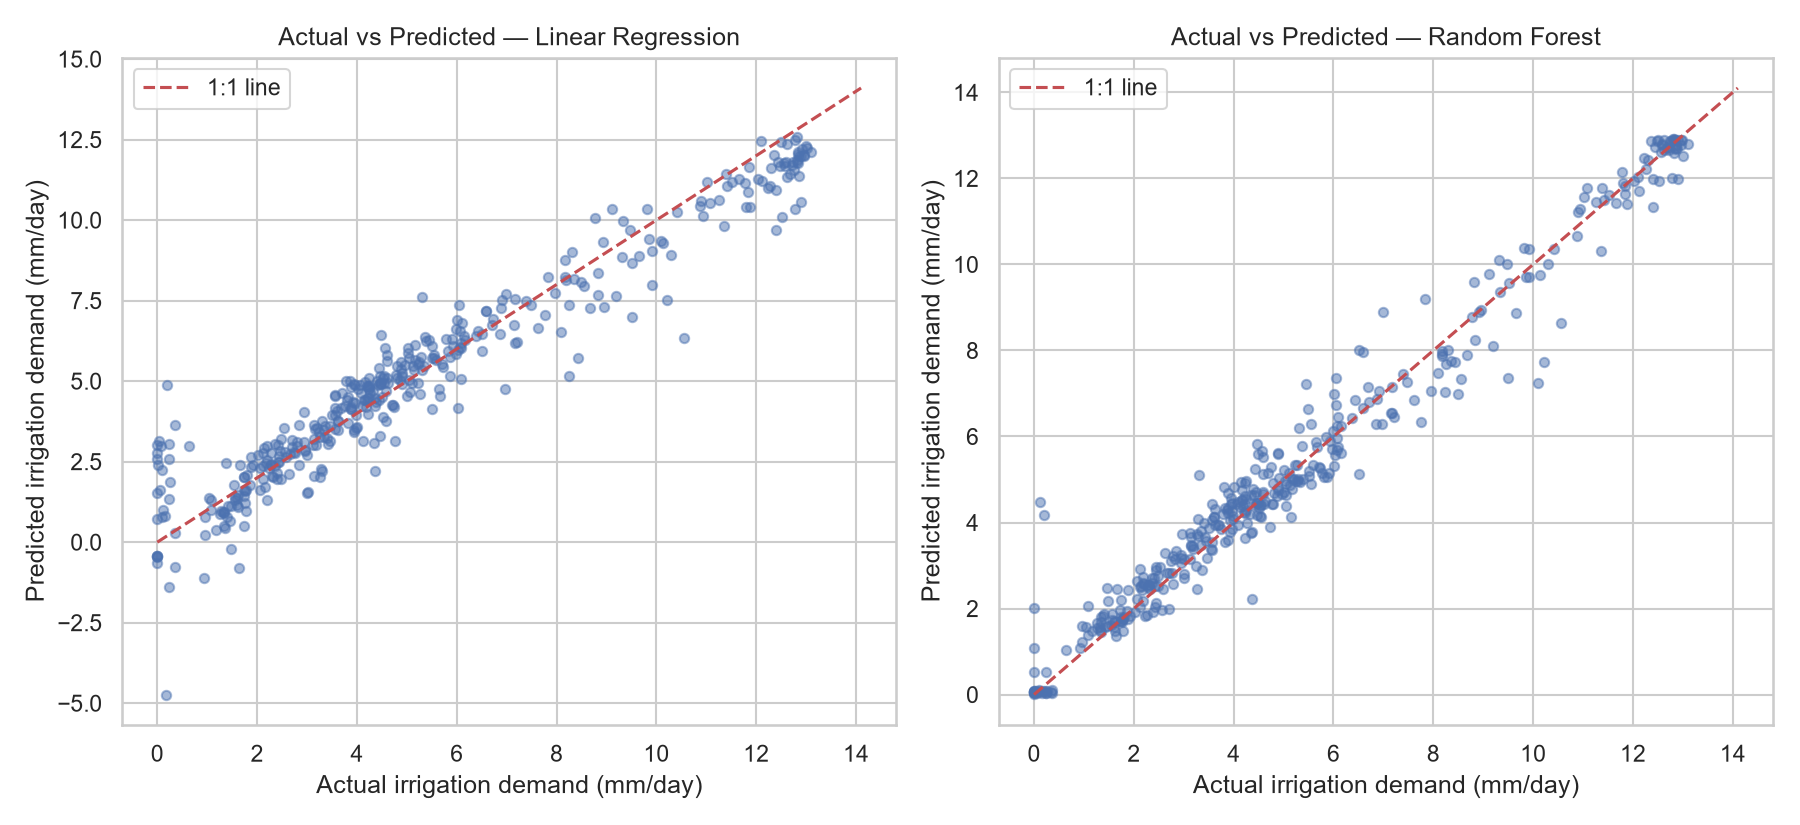
\includegraphics[width=\textwidth]{../figures/05_actual_vs_predicted.png}
\caption{Actual vs.\ predicted irrigation demand --- Linear Regression (left) vs.\ Random Forest (right). Note Linear Regression's occasional physically-impossible negative predictions.}
\label{fig:actual-vs-predicted}
\end{figure}

\begin{figure}[H]
\centering
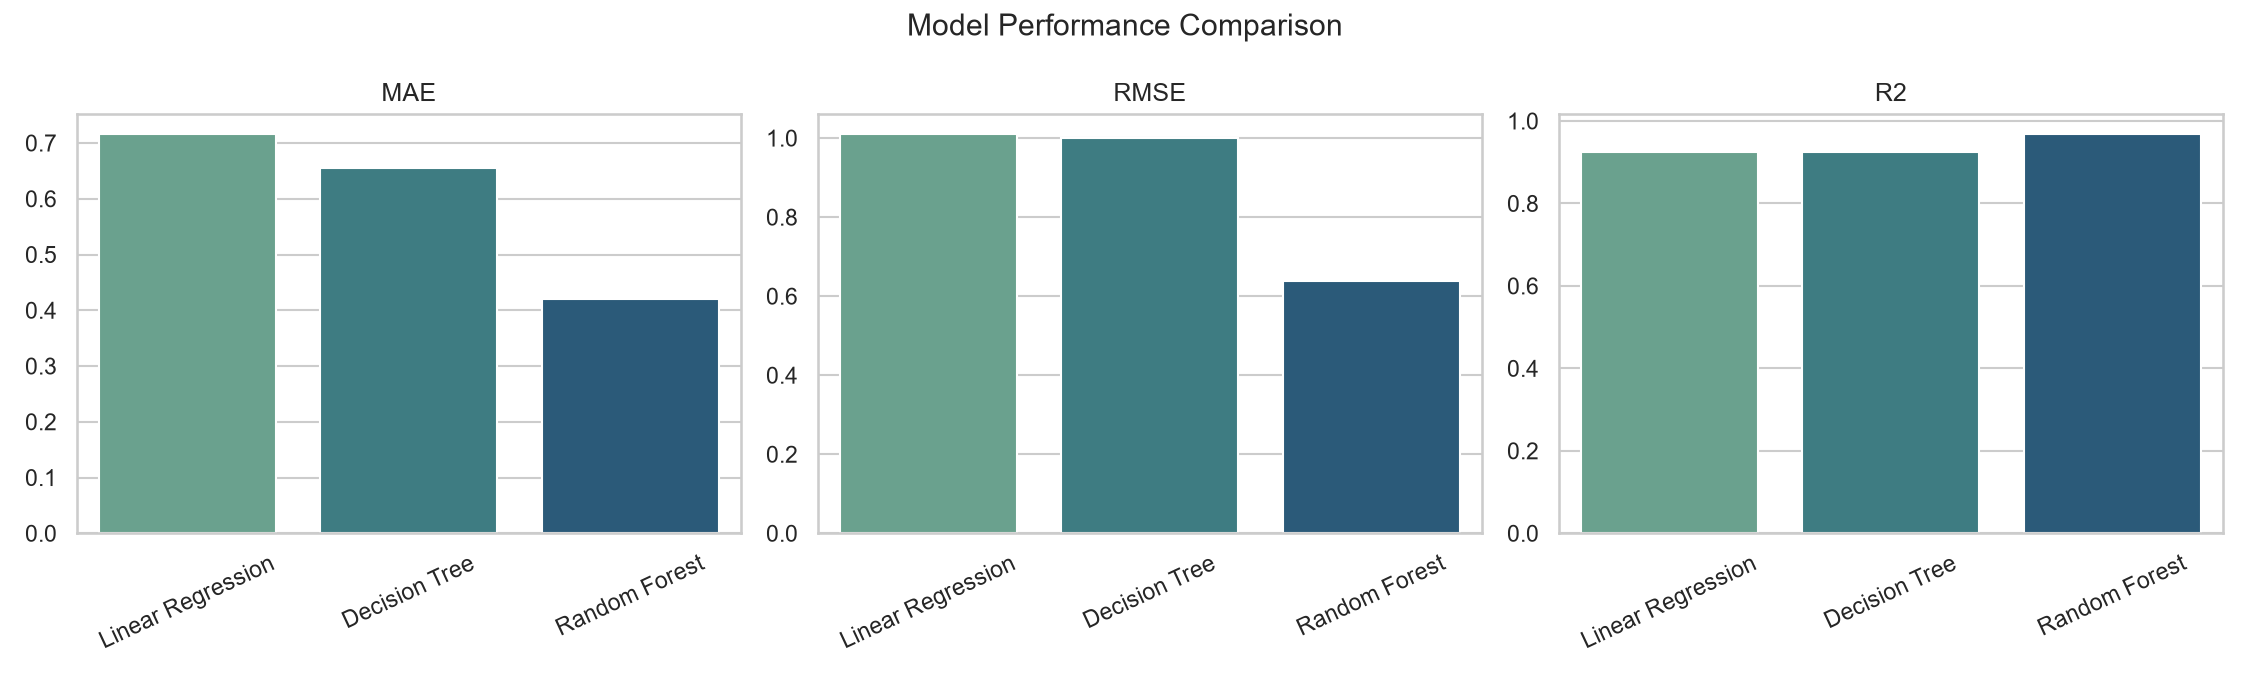
\includegraphics[width=0.9\textwidth]{../figures/06_model_comparison.png}
\caption{Model performance comparison across MAE, RMSE, and R\textsuperscript{2}.}
\label{fig:model-comparison}
\end{figure}

\section{Feature Importance --- Three Complementary Metrics}

A single importance metric can be misleading, so this project computes and
cross-checks \textbf{three independent measures}:

\begin{enumerate}[label=\arabic*.,leftmargin=2em]
    \item \textbf{Correlation with target} --- the simplest possible measure:
    raw Pearson correlation between each feature and
    \texttt{irrigation\_demand\_mm} across the full dataset. Ignores every
    other feature and any nonlinearity, but is a useful sanity-check baseline.
    \item \textbf{Random Forest MDI importance} (Mean Decrease in Impurity)
    --- how much each feature reduced prediction variance, summed across
    every split in every tree, normalized to sum to 1. Reflects how often and
    how effectively a feature was used to build the trees, using only the
    \emph{training} data.
    \item \textbf{Permutation importance} --- the most direct answer to
    ``what feature was actually important \textbf{for prediction}'': take the
    trained Random Forest, shuffle one feature column at a time in the
    \textbf{held-out test set}, and measure how much the model's
    R\textsuperscript{2} \emph{drops}. Computed on the test set, so it
    directly measures each feature's contribution to \emph{generalizing}
    (out-of-sample) prediction accuracy, not just how it was used to fit the
    training data.
\end{enumerate}

\begin{table}[H]
\centering
\caption{Feature importance --- three complementary metrics}
\label{tab:importance}
\begin{tabular}{@{}lccc@{}}
\toprule
\textbf{Feature} & \textbf{Correlation} & \textbf{RF MDI} & \textbf{RF permutation} \\
& \textbf{with target} & \textbf{importance} & \textbf{importance (mean $\pm$ std)} \\
\midrule
\texttt{previous\_irrigation\_mm} & 0.840 & 0.713 & \textbf{0.579 $\pm$ 0.040} \\
\texttt{crop\_coefficient} & 0.551 & 0.107 & 0.222 $\pm$ 0.014 \\
\texttt{rainfall\_mm} & $-0.404$ & 0.106 & 0.170 $\pm$ 0.016 \\
\texttt{solar\_radiation\_MJ\_m2\_day} & 0.658 & 0.033 & 0.058 $\pm$ 0.008 \\
\texttt{temperature\_C} & 0.360 & 0.016 & 0.030 $\pm$ 0.003 \\
\texttt{humidity\_percent} & $-0.563$ & 0.012 & 0.026 $\pm$ 0.003 \\
\texttt{wind\_speed\_mps} & $-0.024$ & 0.012 & 0.019 $\pm$ 0.002 \\
\texttt{growth\_stage} & 0.385 & 0.001 & $\approx$0.000 \\
\bottomrule
\end{tabular}
\end{table}

\begin{figure}[H]
\centering
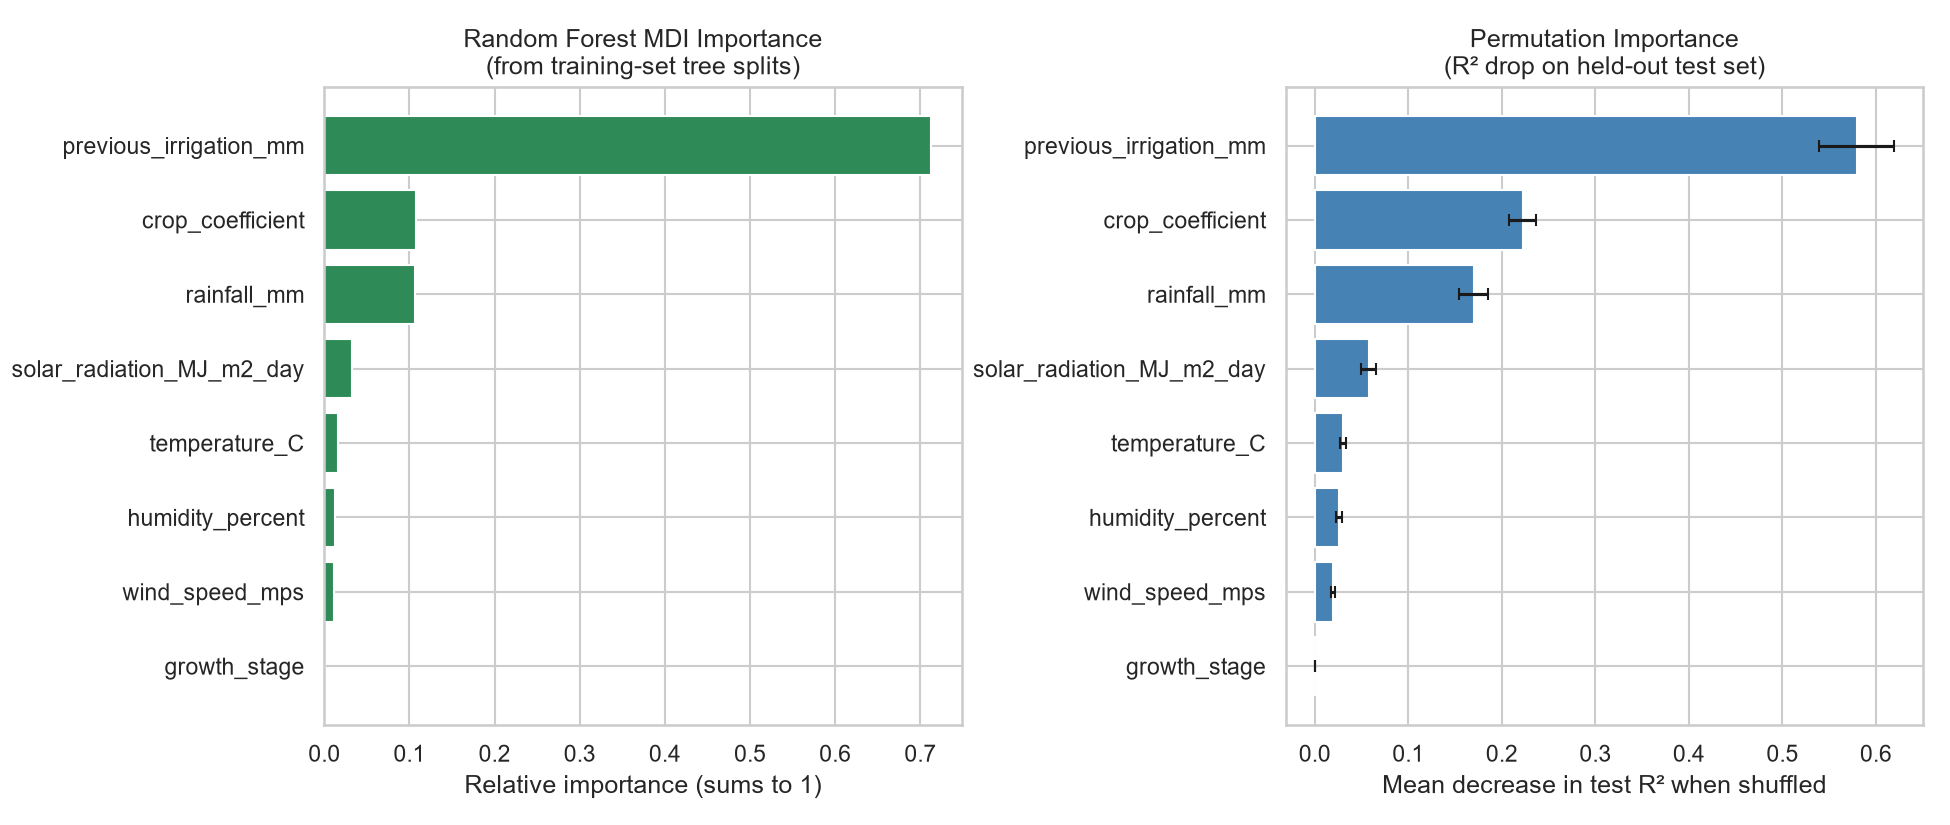
\includegraphics[width=\textwidth]{../figures/07_feature_importance_comparison.png}
\caption{Random Forest MDI importance (left) vs.\ permutation importance on the held-out test set (right). Error bars show $\pm 1$ standard deviation across 30 repeated shufflings.}
\label{fig:feature-importance}
\end{figure}

\textbf{Interpretation:}

\begin{itemize}[leftmargin=2em]
    \item \texttt{previous\_irrigation\_mm} dominates \textbf{all three}
    metrics because the underlying weather is strongly \textbf{autocorrelated
    day-to-day} (heatwaves and wet spells persist for several days) ---
    yesterday's demand is already a strong proxy for today's, a well-known
    \textbf{persistence effect} in hydro-meteorological forecasting. This is a
    genuine feature of the data-generating process, not a modelling artefact,
    but it does mean the model is partly leaning on autocorrelation rather
    than ``understanding'' the weather-to-demand mapping from scratch each
    day.
    \item \texttt{crop\_coefficient} and \texttt{rainfall\_mm} rank next on
    every metric, and sensibly so: both terms enter the FAO-56 water balance
    \textbf{directly and multiplicatively/subtractively}
    ($ET_c = ET_0 \times K_c$; $\text{Net} = ET_c - P_e$), whereas
    temperature/humidity/wind/solar radiation only act \emph{indirectly},
    combined nonlinearly inside the Penman--Monteith ET$_0$ calculation.
    \item \textbf{MDI and permutation importance broadly agree}, which is an
    important cross-check: MDI can sometimes overstate the importance of
    continuous features purely because they offer more possible split
    points, but since permutation importance --- measured completely
    differently, directly on held-out prediction accuracy --- tells the same
    story, the ranking is not an artefact of one particular method.
    \item \texttt{growth\_stage}'s near-zero importance on every metric is
    not a failure --- \texttt{crop\_coefficient} already encodes the same
    underlying information (and does so more precisely, as a continuous
    value), so the model correctly treats \texttt{growth\_stage} as
    redundant.
    \item The permutation-importance \textbf{error bars} (standard deviation
    across 30 repeated shufflings) show that \texttt{previous\_irrigation\_mm}'s
    effect is both large and highly consistent, whereas several of the weaker
    weather features have importances close to (or overlapping) zero once
    repeat-to-repeat variability is accounted for --- their individual
    predictive contribution, once the stronger features are already in the
    model, is genuinely small, not just small-but-uncertain.
\end{itemize}

\section{Discussion --- Are the Results Physically Reasonable?}

Yes, on three independent checks:

\begin{enumerate}[label=\arabic*.,leftmargin=2em]
    \item \textbf{Seasonal pattern.} Monthly-average irrigation demand peaks
    in March--May (hot, dry, pre-monsoon: $\sim$7.4, 11.2, 8.5~mm/day
    respectively) and drops sharply through the monsoon (June--October:
    $\sim$3.0--4.3~mm/day), rising moderately again in winter
    ($\sim$3--4.4~mm/day) --- this reproduces the well-established Indian
    agro-climatic irrigation calendar, where irrigation is most critical
    exactly when it is driest and hottest (Figure~\ref{fig:monthly}).
    \item \textbf{Feature importance ranking.} All three importance metrics
    agree that variables entering the FAO-56 water balance directly ($K_c$,
    rainfall) outrank variables that act only indirectly through ET$_0$ ---
    consistent with the physics used to construct the data.
    \item \textbf{No systematic bias.} Actual and predicted means agree
    closely for every model; errors are concentrated in day-to-day precision
    (captured by MAE/RMSE), not a directional bias.
\end{enumerate}

\begin{figure}[H]
\centering
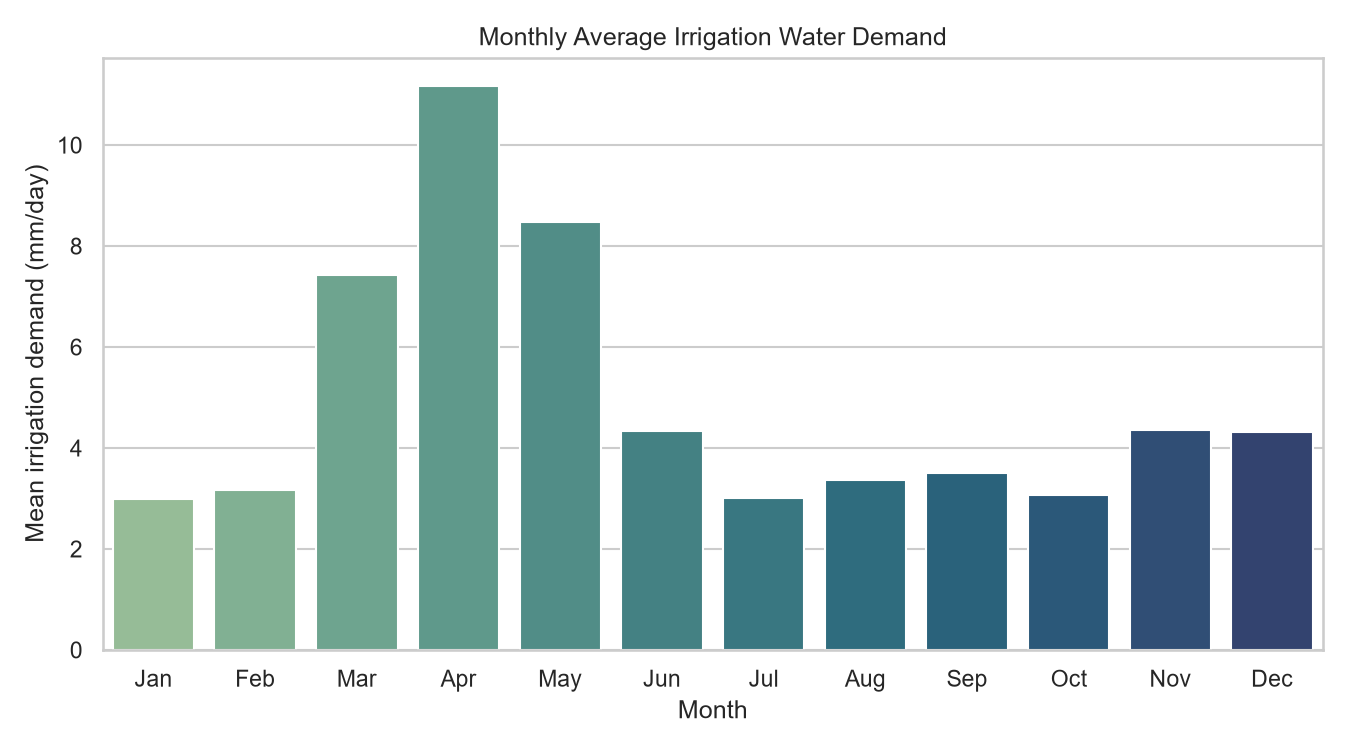
\includegraphics[width=0.8\textwidth]{../figures/08_monthly_avg_demand.png}
\caption{Monthly average irrigation water demand, reproducing the expected Indian agro-climatic irrigation calendar.}
\label{fig:monthly}
\end{figure}

The one caveat worth flagging honestly: the heavy reliance on
\texttt{previous\_irrigation\_mm} means the reported accuracy partly reflects
the persistence/autocorrelation structure of the (synthetic) weather rather
than the model having learned the full weather$\rightarrow$ET$_0$
$\rightarrow$demand chain from first principles. A model trained without this
feature would give a cleaner test of ``pure'' weather-to-demand learning (see
Section~\ref{sec:limitations}).

\section{Limitations and Future Scope}
\label{sec:limitations}

\begin{enumerate}[label=\arabic*.,leftmargin=2em]
    \item \textbf{Synthetic, not observed, data.} Internally consistent with
    FAO-56 physics, but never validated against a real instrumented field.
    Real fields add soil heterogeneity, imperfect irrigation application
    efficiency, and pest/disease effects on $K_c$ not modelled here.
    \item \textbf{Single crop, single location.} Only maize at one
    representative central-Indian climate is modelled; other crops/regions
    would need their own FAO-56 $K_c$ values and climatology.
    \item \textbf{Daily application of a monthly effective-rainfall formula}
    (USDA-SCS) --- an explicit, documented simplification.
    \item \textbf{Continuous back-to-back cropping} (no fallow period between
    harvest and re-sowing) was assumed for simplicity; real fields have
    fallow/rotation gaps.
    \item \textbf{Dominance of the persistence feature}
    (\texttt{previous\_irrigation\_mm}), confirmed by all three
    feature-importance metrics --- future work should retrain without it to
    isolate genuine weather-to-demand predictive skill, relevant for
    multi-day-ahead forecasts where yesterday's true value is unavailable.
    \item \textbf{No deep learning / sequence models} (e.g., LSTM) were used,
    per the project's intended undergraduate scope; comparing against these
    would be a natural extension.
    \item \textbf{No real-time soil-moisture or market data feed} --- a
    deployed system would need this to correct for the gap between
    calculated and true field water status.
\end{enumerate}

\section{Conclusion}

This project built and validated a complete pipeline --- from FAO-56 physical
first principles through synthetic dataset generation to machine-learning
prediction --- for daily irrigation water demand. The Random Forest model
substantially outperformed a linear baseline
(R\textsuperscript{2} $\approx$ 0.97 vs.\ 0.92; MAE $\approx$ 0.42 vs.\
0.72~mm/day), confirming that irrigation demand is governed by nonlinear
interactions among weather, crop coefficient, and rainfall --- directly
traceable to the nonlinear structure of the Penman--Monteith equation and the
FAO-56 crop water balance used to generate the data. A three-metric
feature-importance analysis (correlation, MDI, and permutation importance)
consistently identified antecedent demand, crop coefficient, and rainfall as
the dominant predictors, cross-validating the ranking across independent
methods rather than relying on a single, potentially misleading measure. The
results pass multiple physical-reasonableness checks (correct seasonal
pattern, sensible feature importance ranking, no systematic bias),
demonstrating that a modest, well-engineered feature set and standard
scikit-learn regressors are sufficient for an undergraduate-level
machine-learning approach to irrigation scheduling support.

\begin{thebibliography}{9}

\bibitem{fao56}
Allen, R.G., Pereira, L.S., Raes, D., Smith, M. (1998).
\textit{Crop Evapotranspiration -- Guidelines for Computing Crop Water
Requirements.} FAO Irrigation and Drainage Paper No. 56. Food and Agriculture
Organization of the United Nations, Rome.

\bibitem{fao25}
Doorenbos, J., Pruitt, W.O. (1977).
\textit{Guidelines for Predicting Crop Water Requirements.}
FAO Irrigation and Drainage Paper No. 24/25. FAO, Rome.

\bibitem{usda-scs}
USDA Soil Conservation Service (1970).
\textit{Irrigation Water Requirements.}
Technical Release No. 21, USDA-SCS, Washington, D.C.

\bibitem{imd}
India Meteorological Department (IMD) --- representative climatological
normals for central India, used only to loosely calibrate synthetic monthly
weather ranges.

\bibitem{rf}
Breiman, L. (2001).
Random Forests.
\textit{Machine Learning}, 45(1), 5--32.

\bibitem{permimp}
Fisher, A., Rudin, C., Dominici, F. (2019).
All Models are Wrong, but Many are Useful: Learning a Variable's Importance
by Studying an Entire Class of Prediction Models Simultaneously.
\textit{Journal of Machine Learning Research}, 20(177), 1--81.

\bibitem{sklearn}
Pedregosa, F., Varoquaux, G., Gramfort, A., et al. (2011).
Scikit-learn: Machine Learning in Python.
\textit{Journal of Machine Learning Research}, 12, 2825--2830.

\bibitem{pandas}
McKinney, W. (2010).
Data Structures for Statistical Computing in Python.
\textit{Proceedings of the 9th Python in Science Conference}, 51--56.

\end{thebibliography}

\vspace{1em}
\noindent\rule{\textwidth}{0.4pt}

\vspace{0.5em}
\noindent\footnotesize\emph{Note on data provenance: all daily weather and
irrigation-demand observations in this report are synthetically generated
(Section 3.2), using FAO-56-based relationships calibrated to realistic Indian
agricultural weather ranges. They are not measurements from any real farm,
field trial, or government meteorological station. All model metrics
(Section 5) and feature-importance figures (Section 6) were obtained by
actually training the described models and running the described analyses on
this generated dataset (\texttt{model\_training.ipynb}, reproducible with
\texttt{random\_state=42}) --- none were fabricated in advance.}

\end{document}
